\chapter{Potencial químico y mezclas}\label{ch:b2:chemical-potential}

En invierno un camión esparce sal sobre una carretera helada y el hielo se funde a
\qty{-10}{\celsius}; el líquido refrigerante de un motor de coche, agua con un tercio de
etano-1,2-diol, ni se congela con la helada nocturna ni hierve bajo un capó
caliente. Una sustancia disuelta rebaja el punto de congelación de su disolvente y
eleva su punto de ebullición y, en disoluciones diluidas, lo hace en una cantidad que
depende del número de partículas disueltas y no de su naturaleza. La
herramienta que lo explica es el \omterm{def:b2:chemical-potential:chemical-potential}{potencial químico}, la derivada parcial de
la \omterm{def:b2:reaction-free-energy:gibbs-energy}{energía de Gibbs} respecto de la cantidad de un constituyente. Indica
adónde ``quiere ir'' cada especie, entre fases y a través de reacciones,
y convierte las actividades que el volumen del primer año usaba como recetas en
magnitudes deducidas.

\begin{recall}
\Cref{ch:b2:reaction-free-energy}: la \omterm{def:b2:reaction-free-energy:gibbs-energy}{energía de Gibbs} $G = H - TS$, $\dd G =
V\dd p - S\dd T + \Delta_r G\,\dd\xi$, el criterio de evolución $\Delta_r G\,
\dd\xi \leq 0$. El volumen del primer año escribió la actividad de un gas como
$p_i/p^\circ$, la de un soluto como $c_i/c^\circ$, y 1 para un sólido puro o un
disolvente, y señaló que en las disoluciones iónicas concentradas las actividades se alejan
de las concentraciones, ``una corrección que se deja para el volumen del segundo año''. De la
física: la ley de los gases perfectos, y $(\partial G/\partial p)_T = V$ para una
sustancia pura.
\end{recall}

\begin{omfigure}

\includegraphics[width=0.58\linewidth]{images/book3/ai/b2-03-salt-spreader.jpg}

{\small Un camión esparcidor de sal en una carretera nevada. La sal se disuelve
en la fina película de agua sobre el hielo, y la disolución se congela a una
temperatura más baja que el agua pura: el hielo se funde.}
\end{omfigure}

\section{Magnitudes molares parciales}

Mézclense \qty{50}{mL} de agua y \qty{50}{mL} de etanol: el volumen de la
mezcla es inferior a \qty{100}{mL}. En una mezcla, una magnitud extensiva no es
la suma de las contribuciones de las sustancias puras; cada constituyente
contribuye según su entorno.

\begin{definition}[Magnitud molar parcial]\label{def:b2:chemical-potential:partial-molar}
Sea $X(T, p, n_1, \dots, n_k)$ una función de estado extensiva de una fase
que contiene las cantidades $n_1, \dots, n_k$. La \emph{magnitud molar
parcial}\index{magnitud molar parcial} del constituyente $i$ es
\[
  \bar X_i = \left(\frac{\partial X}{\partial n_i}\right)_{T, p, n_{j \ne i}} ,
\]
la variación de $X$ por mol de $i$ añadido a una gran cantidad de mezcla
a $T$, $p$ y demás cantidades fijas. Para $X = V$ es el \emph{volumen
molar parcial}\index{volumen molar parcial} $\bar V_i$.
\end{definition}

\begin{theorem}[Identidad de Euler]\label{thm:b2:chemical-potential:euler}
A $T$ y $p$ fijas, $X = \sum_i n_i\bar X_i$.
\end{theorem}

\begin{proof}
$X$ es extensiva: al multiplicar todas las cantidades por $\lambda$, también $X$ queda multiplicada por
$\lambda$, $X(T, p, \lambda n_1, \dots, \lambda n_k) = \lambda X(T, p, n_1,
\dots, n_k)$. Derivando respecto de $\lambda$ en $\lambda = 1$, con
la regla de la cadena: $\sum_i n_i\,\partial X/\partial n_i = X$.
\end{proof}

\begin{proposition}[Relación de Gibbs--Duhem]\label{prop:b2:chemical-potential:gibbs-duhem}
A $T$ y $p$ fijas, $\sum_i n_i\,\dd\bar X_i = 0$: en una mezcla binaria,
$x_1\dd\bar X_1 + x_2\dd\bar X_2 = 0$. Las \omterm{def:b2:chemical-potential:partial-molar}{magnitudes molares parciales} de los
constituyentes no pueden variar de forma independiente.
\end{proposition}

\begin{proof}
A $T$ y $p$ fijas, $\dd X = \sum_i\bar X_i\dd n_i$ por definición; la identidad de
Euler, diferenciada, da $\dd X = \sum_i\bar X_i\dd n_i + \sum_i
n_i\dd\bar X_i$. Se restan.
\end{proof}

\begin{omfigure}
\begin{tikzpicture}
\begin{axis}[
  width=0.62\linewidth, height=5.4cm, xmin=0, xmax=1, ymin=8, ymax=62,
  axis x line=bottom, axis y line=left, xlabel={fracción molar $x_2$},
  ylabel={volumen molar $V_m$ (modelo)}, xtick={0,0.2,0.4,0.6,0.8,1}, ytick=\empty,
  tick label style={font=\small}, label style={font=\small}, ylabel shift=10pt, clip=false]
\addplot[omDef, very thick, domain=0:1, samples=60] {18*(1-x) + 58*x - 25*x*(1-x)};
\addplot[black!40, dashed, domain=0:1] {18*(1-x) + 58*x};
\addplot[omThm, thick, domain=0:1] {14 + 35*x};
\fill[omThm] (axis cs:0.4,28) circle (1.6pt);
\node[omThm, anchor=east, font=\small] at (axis cs:-0.01,14) {$\bar V_1$};
\node[omThm, anchor=west, font=\small] at (axis cs:1,49) {$\bar V_2$};
\node[font=\scriptsize, anchor=south east, black!60] at (axis cs:0.62,44) {suma de los volúmenes puros};
\node[font=\small, anchor=north west] at (axis cs:0.41,27) {$x_2 = 0.4$};
\end{axis}
\end{tikzpicture}

{\small La construcción de la tangente. El volumen molar de una mezcla binaria modelo
(azul) queda por debajo de la recta que une los volúmenes puros: la mezcla
se contrae. La tangente en una composición corta los dos bordes en los volúmenes
molares parciales $\bar V_1$ y $\bar V_2$ de esa composición.}
\end{omfigure}

\begin{method}[Magnitudes molares parciales a partir de una curva]\label{met:b2:chemical-potential:tangent}
Represéntese la magnitud molar $X_m = X/(n_1 + n_2)$ frente a $x_2$. En la
composición que interesa trácese la tangente: corta el eje $x_2 = 0$ en
$\bar X_1$ y el eje $x_2 = 1$ en $\bar X_2$. (Demostración: $X_m = x_1\bar X_1 +
x_2\bar X_2$ y, por Gibbs--Duhem, $\dd X_m/\dd x_2 = \bar X_2 - \bar X_1$.)
\end{method}

\section{El potencial químico}

\begin{definition}[Potencial químico]\label{def:b2:chemical-potential:chemical-potential}
El \emph{potencial químico}\index{potencial quimico@potencial químico} del constituyente $i$ en
una fase es su \omterm{def:b2:reaction-free-energy:gibbs-energy}{energía de Gibbs} molar parcial,
\[
  \mu_i = \left(\frac{\partial G}{\partial n_i}\right)_{T, p, n_{j\ne i}} ,
\]
en \unit{J/mol}. Su valor cuando $i$ está en su estado estándar es su
\emph{potencial químico estándar}\index{potencial quimico estandar@potencial químico estándar}
$\mu_i^\circ(T)$, igual a la \omterm{def:b2:reaction-free-energy:gibbs-energy}{energía de Gibbs} molar estándar de $i$.
\end{definition}

Para una fase cuyas cantidades pueden cambiar (por reacción o por intercambio con
otra fase),
\[
  \dd G = V\dd p - S\dd T + \sum_i\mu_i\,\dd n_i ,\qquad G = \sum_i n_i\mu_i ,
\]
la segunda relación por la identidad de Euler. Con una sola reacción, $\dd n_i =
\nu_i\dd\xi$, y comparando con la \cref{prop:b2:reaction-free-energy:dG}:
\[
  \Delta_r G = \sum_i\nu_i\mu_i .
\]
La \omterm{def:b2:reaction-free-energy:reaction-gibbs}{energía de Gibbs de reacción} es el balance de los \omterm{def:b2:chemical-potential:chemical-potential}{potenciales químicos} de los
productos y de los reactivos.

\begin{theorem}[Equilibrio entre fases]\label{thm:b2:chemical-potential:phase-equilibrium}
Un constituyente presente en dos fases $\alpha$ y $\beta$ de un sistema cerrado a
$T$ y $p$ uniformes está en equilibrio entre ellas si y solo si
$\mu_i^\alpha = \mu_i^\beta$. En caso contrario pasa espontáneamente de la
fase donde su \omterm{def:b2:chemical-potential:chemical-potential}{potencial químico} es más alto a la fase donde es más bajo.
\end{theorem}

\begin{proof}
La transferencia $i^\alpha \to i^\beta$ es una ``reacción'' con $\nu^\alpha = -1$,
$\nu^\beta = +1$, luego $\Delta_r G = \mu_i^\beta - \mu_i^\alpha$. Por el
criterio de evolución avanza ($\dd\xi > 0$) solo si $\mu_i^\beta <
\mu_i^\alpha$, retrocede si $\mu_i^\beta > \mu_i^\alpha$, y está en
equilibrio si son iguales.
\end{proof}

El \omterm{def:b2:chemical-potential:chemical-potential}{potencial químico} desempeña para la materia el papel que la temperatura desempeña
para el calor: el calor fluye de lo caliente a lo frío, una especie, de donde su $\mu$ es alto a donde es bajo.

\section{Sistemas ideales y actividades}

\begin{proposition}[Potencial químico de un gas perfecto]\label{prop:b2:chemical-potential:mu-gas}
En una mezcla de gases perfectos, un gas de presión parcial $p_i$ tiene
\[
  \mu_i = \mu_i^\circ(T) + RT\ln\frac{p_i}{p^\circ} .
\]
\end{proposition}

\begin{proof}
Para un mol de un gas perfecto puro, $(\partial\mu/\partial p)_T = V_m =
RT/p$; integrando de $p^\circ$ a $p$ se obtiene $\mu = \mu^\circ + RT\ln(p/p^\circ)$.
En una mezcla de gases perfectos cada gas se comporta como si estuviera solo en el volumen, a
su presión parcial: se sustituye $p$ por $p_i$.
\end{proof}

\begin{definition}[Mezcla ideal, disolución diluida ideal]\label{def:b2:chemical-potential:ideal-mixture}
Una mezcla líquida (o sólida) es una \emph{mezcla ideal}\index{mezcla ideal}
si, para todo constituyente y toda composición,
$\mu_i = \mu_i^*(T, p) + RT\ln x_i$, donde $\mu_i^*$ es el \omterm{def:b2:chemical-potential:chemical-potential}{potencial químico}
del líquido puro $i$. Una disolución es una \emph{disolución diluida
ideal}\index{disolucion diluida ideal@disolución diluida ideal} si el disolvente obedece esta ley y cada
soluto obedece $\mu_j = \mu_j^\circ(T) + RT\ln(c_j/c^\circ)$, con un estado
estándar que es una disolución hipotética a $c^\circ = \qty{1}{mol/L}$ que se comporta
como si estuviera infinitamente diluida.
\end{definition}

Las moléculas de tamaño y forma parecidos cuyas interacciones no dependen de
la pareja (benceno y tolueno, dos formas isotópicas de una molécula) forman
mezclas casi ideales; las disoluciones diluidas se comportan idealmente porque cada partícula de
soluto está rodeada solo de disolvente.

\begin{theorem}[Ley de Raoult]\label{thm:b2:chemical-potential:raoult}
Sobre una mezcla líquida ideal, con el vapor como gas perfecto, la presión
parcial de cada constituyente es proporcional a su fracción molar en el
líquido: $p_i = x_i\,p_i^*$, donde $p_i^*$ es la presión de vapor del líquido
puro a la misma temperatura (\emph{ley de Raoult}\index{ley de Raoult}).
\end{theorem}

\begin{proof}
En el equilibrio $\mu_i(\text{líquido}) = \mu_i(\text{vapor})$: $\mu_i^* +
RT\ln x_i = \mu_i^\circ + RT\ln(p_i/p^\circ)$. Para el líquido puro ($x_i = 1$,
$p_i = p_i^*$): $\mu_i^* = \mu_i^\circ + RT\ln(p_i^*/p^\circ)$. Restando,
$RT\ln x_i = RT\ln(p_i/p_i^*)$. (Se desprecia la débil dependencia de $\mu_i^*$ con la
presión.)
\end{proof}

\begin{proposition}[Ley de Henry]\label{prop:b2:chemical-potential:henry}
Para un soluto diluido $j$ en equilibrio con su vapor, $p_j = k_{H,j}\,x_j$
(o $c_j = H_j\,p_j$): la presión parcial de un soluto diluido es
proporcional a su cantidad en la disolución (\emph{ley de
Henry}\index{ley de Henry}). La \emph{constante de Henry}\index{constante de Henry}
$k_{H,j}$ depende del soluto, del disolvente y de la temperatura, y no es
la presión de vapor del soluto puro.
\end{proposition}

\begin{proof}
Se igualan $\mu_j^\circ(\text{disolución}) + RT\ln(c_j/c^\circ)$ y
$\mu_j^\circ(\text{gas}) + RT\ln(p_j/p^\circ)$: $c_j/p_j$ es función solo de $T$.
La constante contiene las interacciones de $j$ con el disolvente, no
consigo mismo.
\end{proof}

\begin{omfigure}
\begin{tikzpicture}
\begin{axis}[name=a,
  width=0.48\linewidth, height=5.6cm, xmin=0, xmax=1, ymin=0, ymax=1.5,
  axis x line=bottom, axis y line=left, xlabel={$x_1$}, ylabel={$p/p_1^*$},
  xtick={0,0.5,1}, ytick={0,0.5,1,1.5},
  tick label style={font=\small}, label style={font=\small}, title={\small ideal}]
\addplot[omDef, thick] table[x=x1, y=p1] {figdata/out/bachelor-2-raoult-henry-ideal.dat};
\addplot[omThm, thick] table[x=x1, y=p2] {figdata/out/bachelor-2-raoult-henry-ideal.dat};
\addplot[black, very thick] table[x=x1, y=p] {figdata/out/bachelor-2-raoult-henry-ideal.dat};
\node[omDef, font=\scriptsize, anchor=west] at (axis cs:0.55,0.42) {$p_1$};
\node[omThm, font=\scriptsize, anchor=west] at (axis cs:0.1,0.42) {$p_2$};
\node[font=\scriptsize, anchor=south] at (axis cs:0.5,0.8) {$p$};
\end{axis}
\begin{axis}[at={(a.east)}, anchor=west, xshift=1.2cm,
  width=0.48\linewidth, height=5.6cm, xmin=0, xmax=1, ymin=0, ymax=1.5,
  axis x line=bottom, axis y line=left, xlabel={$x_1$},
  xtick={0,0.5,1}, ytick={0,0.5,1,1.5},
  tick label style={font=\small}, label style={font=\small}, title={\small desviación positiva}]
\addplot[omDef, thick] table[x=x1, y=p1] {figdata/out/bachelor-2-raoult-henry-margules.dat};
\addplot[omThm, thick] table[x=x1, y=p2] {figdata/out/bachelor-2-raoult-henry-margules.dat};
\addplot[black, very thick] table[x=x1, y=p] {figdata/out/bachelor-2-raoult-henry-margules.dat};
\addplot[omDef, densely dashed, domain=0.6:1] {x};
\addplot[omDef, dotted, thick, domain=0:0.42] {3.004166*x};
\node[omDef, font=\scriptsize, anchor=west] at (axis cs:0.62,0.5) {Raoult};
\node[omDef, font=\scriptsize, anchor=east] at (axis cs:0.27,1.18) {Henry};
\node[omDef, font=\scriptsize, anchor=north west] at (axis cs:0.8,0.78) {$p_1$};
\node[omThm, font=\scriptsize, anchor=north] at (axis cs:0.55,0.24) {$p_2$};
\node[font=\scriptsize, anchor=south] at (axis cs:0.5,1.23) {$p$};
\end{axis}
\end{tikzpicture}

{\small Presiones de vapor sobre un líquido binario a temperatura fija, en unidades
de $p_1^*$ (mezcla modelo). A la izquierda, una \omterm{def:b2:chemical-potential:ideal-mixture}{mezcla ideal}: rectas (Raoult).
A la derecha, una mezcla cuyas moléculas distintas se atraen menos que las
iguales: las presiones quedan por encima de las rectas ideales. Cerca de $x_1 = 1$, el constituyente 1
sigue la recta de Raoult (discontinua); cerca de $x_1 = 0$, sigue una recta de Henry
(punteada) de otra pendiente.}
% (computed in figdata/bachelor-2/raoult-henry.py; Margules parameter 1.1, model)
\end{omfigure}

\begin{example}[El dióxido de carbono de un refresco]\label{ex:b2:chemical-potential:soda}
A \qty{25}{\celsius} la \omterm{prop:b2:chemical-potential:henry}{constante de Henry} del dióxido de carbono en agua es $H =
\qty{3.4e-4}{mol/(m^3.Pa)}$, es decir, \qty{0.034}{mol/(L.bar)}. Una botella
cerrada bajo \qty{4}{bar} de \ce{CO2} contiene $0.034 \times 4 =
\qty{0.14}{mol/L}$ de gas disuelto, unos \qty{6}{g/L}. Abierta, el gas
sobre ella es el aire, donde $p_{\ce{CO2}} \approx \qty{4e-4}{bar}$: la bebida está
diez mil veces sobresaturada y burbujea hasta quedarse sin gas.
% ledger: henry:CO2, air:CO2
\end{example}

\begin{proposition}[Actividades a partir de los potenciales químicos]\label{prop:b2:chemical-potential:activity}
En todos los casos vistos hasta ahora, $\mu_i = \mu_i^\circ(T) + RT\ln a_i$, donde $a_i$
es la actividad del volumen del primer año: $p_i/p^\circ$ para un gas perfecto,
$c_i/c^\circ$ para un soluto en una \omterm{def:b2:chemical-potential:ideal-mixture}{disolución diluida ideal}, $x_i$ (cercana a 1)
para el disolvente, y 1 para un sólido o un líquido puro solo en su fase.
\end{proposition}

\begin{proof}
Para el gas y el soluto diluido es el contenido de la
\cref{prop:b2:chemical-potential:mu-gas} y de la definición de la \omterm{def:b2:chemical-potential:ideal-mixture}{disolución
diluida ideal}. Para un constituyente de una \omterm{def:b2:chemical-potential:ideal-mixture}{mezcla ideal} se toma como estado
estándar el líquido puro: $a_i = x_i$, cercana a 1 para un disolvente. Un sólido
o un líquido puro es su propio estado estándar (despreciando su débil dependencia con la
presión): $\mu = \mu^\circ$, $a = 1$.
\end{proof}

\begin{proposition}[Energía de Gibbs de reacción y cociente]\label{prop:b2:chemical-potential:delta-g-q}
Para una reacción $0 = \sum_i\nu_i\mathrm A_i$,
\[
  \Delta_r G = \Delta_r G^\circ(T) + RT\ln Q, \qquad Q = \prod_i a_i^{\nu_i} .
\]
\end{proposition}

\begin{proof}
$\Delta_r G = \sum_i\nu_i\mu_i = \sum_i\nu_i\mu_i^\circ + RT\sum_i\nu_i\ln a_i =
\Delta_r G^\circ + RT\ln\prod_i a_i^{\nu_i}$.
\end{proof}

Este es el puente entre la \omterm{def:b2:reaction-free-energy:gibbs-energy}{energía de Gibbs} del \cref{ch:b2:reaction-free-energy}
y el cociente de reacción del volumen del primer año. El capítulo siguiente lo cruza.

\begin{method}[Elegir el estado de referencia de una actividad]\label{met:b2:chemical-potential:activity-reference}
\begin{enumerate}
  \item Gas: el gas perfecto puro a $p^\circ$; $a = p_i/p^\circ$.
  \item Disolvente, o constituyente de una mezcla de cantidades comparables: el
        líquido puro; $a = \gamma_i x_i$ (referencia de Raoult, $\gamma_i \to 1$
        cuando $x_i \to 1$).
  \item Soluto: la disolución ideal a $c^\circ$; $a = \gamma_j c_j/c^\circ$
        (referencia de Henry, $\gamma_j \to 1$ a dilución infinita).
  \item Sólido puro, líquido puro solo en su fase: $a = 1$.
\end{enumerate}
\end{method}

\begin{history}[François-Marie Raoult]
\begin{minipage}[t]{0.2\linewidth}\vspace{0pt}
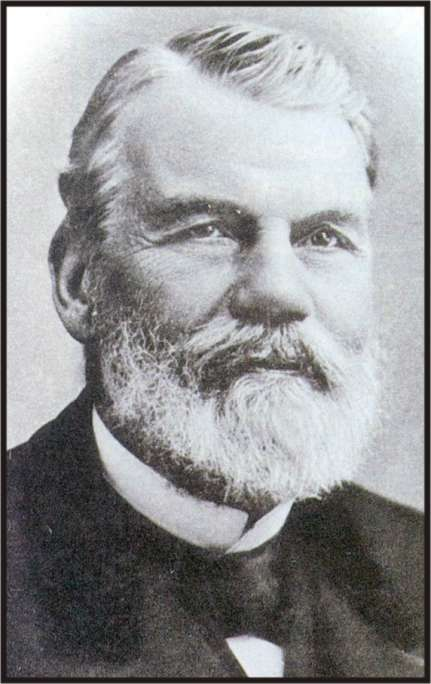
\includegraphics[width=\linewidth]{images/book3/raoult.jpg}
\end{minipage}\hfill
\begin{minipage}[t]{0.76\linewidth}\vspace{0pt}
François-Marie Raoult (1830--1901), profesor de química en Grenoble,
midió durante la década de 1880 los puntos de congelación y luego las presiones de vapor
de cientos de disoluciones, y halló que, para las disoluciones diluidas, el descenso
depende del número de moléculas disueltas y no de su naturaleza. Sus
medidas se convirtieron en un modo de pesar moléculas, y apoyaron la joven
teoría de los iones en disolución. (Fotografía: dominio público, Wikimedia Commons.)
\end{minipage}
\end{history}

\section{Mezclas reales}

\begin{definition}[Coeficiente de actividad]\label{def:b2:chemical-potential:activity-coefficient}
En una mezcla real el \omterm{def:b2:chemical-potential:chemical-potential}{potencial químico} se escribe $\mu_i = \mu_i^\circ +
RT\ln a_i$ con $a_i = \gamma_i x_i$ (referencia de Raoult) o $a_i = \gamma_i
c_i/c^\circ$ (referencia de Henry). El factor $\gamma_i$ es el \emph{coeficiente
de actividad}\index{coeficiente de actividad}: mide la desviación respecto de la
ley ideal, y tiende a 1 en el límite en que se cumple la ley de referencia.
\end{definition}

Un coeficiente mayor que 1 significa que la molécula está menos estabilizada por sus
vecinas en la mezcla que en el estado de referencia (desviación positiva, como en la figura
anterior); menor que 1, más estabilizada. Por Gibbs--Duhem, los coeficientes de los dos
constituyentes de una mezcla binaria están ligados: en el modelo de un parámetro
usado para la figura, $\ln\gamma_1 = Ax_2^2$ y $\ln\gamma_2 = Ax_1^2$, y
$x_1\,\dd\ln\gamma_1 + x_2\,\dd\ln\gamma_2 = 0$ se cumple idénticamente.

Para los iones, que interaccionan a larga distancia, las desviaciones aparecen ya a
concentraciones pequeñas.

\begin{definition}[Fuerza iónica]\label{def:b2:chemical-potential:ionic-strength}
La \emph{fuerza iónica}\index{fuerza ionica@fuerza iónica} de una disolución es $I =
\frac12\sum_i z_i^2\,b_i$, donde $b_i$ es la molalidad del ion $i$ (cantidad por
kilogramo de disolvente) y $z_i$ su número de carga.
\end{definition}

\begin{proposition}[Ley límite de Debye--Hückel]\label{prop:b2:chemical-potential:debye-huckel}
En una disolución de electrolito muy diluida, el \omterm{def:b2:chemical-potential:activity-coefficient}{coeficiente de actividad} medio de los
iones de una sal obedece $\log\gamma_\pm = -A\,|z_+z_-|\sqrt{I/b^\circ}$, con $A
\approx 0.51$ para el agua a \qty{25}{\celsius} y $b^\circ =
\qty{1}{mol/kg}$.
\end{proposition}
\admitted

\begin{remark}[Dominio de validez y origen]\label{rem:b2:chemical-potential:dh-range}
La ley procede de un modelo en el que cada ion está rodeado de una ``atmósfera''
difusa de carga opuesta, que rebaja su \omterm{def:b2:chemical-potential:chemical-potential}{potencial químico}; el
modelo excede este curso, pero su constante $A$ se deduce de la
permitividad y la densidad del agua y de la temperatura. Es precisa por debajo
de aproximadamente $I = \qty{0.01}{mol/kg}$. La misma atmósfera iónica frena los iones en
un campo eléctrico, y explica por qué la conductividad molar de un electrolito
fuerte disminuye según $\Lambda = \Lambda^\circ - K\sqrt c$ (ley de la raíz cuadrada de
Kohlrausch) en lugar de mantenerse en su valor límite: el límite de la
ley de Kohlrausch vista en el volumen del primer año.
% ledger: epsr:H2O, rho:water.298, const:e, const:eps0, const:kB, const:NA (A computed in figdata/bachelor-2/colligative.py)
\end{remark}

\begin{example}[Una sal centimolar]\label{ex:b2:chemical-potential:dh}
Para el cloruro de sodio con $b = \qty{0.010}{mol/kg}$, $I = \frac12(0.010 + 0.010)
= \qty{0.010}{mol/kg}$ y $\log\gamma_\pm = -0.51 \times 0.10$: $\gamma_\pm
= 0.89$. Ya a una centésima de mol por kilogramo, tomar la
concentración por la actividad supone un error del 11\,\%; para una sal 2:2 como
el sulfato de magnesio a la misma molalidad, $I = 0.040$ y $\gamma_\pm = 0.62$.
\end{example}

\section{Propiedades coligativas}

\begin{definition}[Propiedad coligativa]\label{def:b2:chemical-potential:colligative}
Una \emph{propiedad coligativa}\index{propiedad coligativa} de una disolución
diluida es aquella que depende de la cantidad de partículas disueltas por
cantidad de disolvente y no de su naturaleza: el descenso de la presión de
vapor y del punto de congelación, el aumento del punto de ebullición y la
\omterm{def:b2:chemical-potential:osmotic-pressure}{presión osmótica}. Las constantes de las leyes del punto de congelación y del punto de ebullición
que siguen son la \emph{constante crioscópica}\index{constante crioscopica@constante crioscópica} $K_f$
y la \emph{constante ebulloscópica}\index{constante ebulloscopica@constante ebulloscópica} $K_b$ del
disolvente.
\end{definition}

\begin{omfigure}
\begin{tikzpicture}[font=\small, >={Stealth}]
  \draw[->] (0,0) -- (8,0) node[right] {$T$};
  \draw[->] (0,0) -- (0,4.4) node[above] {$\mu$ del disolvente};
  % slopes = -S_m: the liquid, more disordered, falls faster than the solid
  \draw[omDef, very thick] (0.4,3.0) -- (7.0,2.01) node[right] {sólido};
  \draw[omThm, very thick] (0.4,3.6) -- (7.6,0.72) node[right] {líquido puro};
  \draw[omThm, very thick, dashed] (0.4,3.25) -- (7.6,0.37) node[right] {disolución};
  \fill (2.8,2.64) circle (1.5pt);
  \fill (1.4,2.85) circle (1.5pt);
  \draw[densely dotted] (2.8,2.64) -- (2.8,0) node[below] {$T_f^*$};
  \draw[densely dotted] (1.4,2.85) -- (1.4,0) node[below] {$T_f$};
  \draw[<->] (1.4,-0.75) -- (2.8,-0.75) node[midway, below] {$\Delta T_f$};
  \draw[<->, black!70] (5.0,1.76) -- (5.0,1.41);
  \draw[black!50] (5.0,1.58) -- (4.6,0.75) node[below, font=\scriptsize, black] {$RT\ln x_1$};
\end{tikzpicture}

{\small \omterm{def:b2:chemical-potential:chemical-potential}{Potencial químico} del disolvente en función de la temperatura (esquema,
a presión fija). La fase estable es la de $\mu$ más bajo. Disolver un
soluto rebaja la recta del líquido en $RT\ln x_1 < 0$; ahora corta la recta del sólido
a una temperatura más baja: la disolución se congela por debajo del disolvente puro.}
\end{omfigure}

\begin{theorem}[Descenso crioscópico]\label{thm:b2:chemical-potential:cryoscopy}
Una disolución diluida de un soluto que no entra en el sólido empieza a congelarse
a $T_f = T_f^* - \Delta T_f$, con
\[
  \Delta T_f = K_f\,b, \qquad K_f = \frac{R\,T_f^{*2}\,M_1}{\Delta_{\text{fus}}H_1} ,
\]
siendo $b$ la molalidad total de las partículas disueltas y $M_1$ la masa
molar del disolvente (en \unit{kg/mol}). Para concentraciones finitas la relación
exacta para una disolución ideal es $\ln x_1 = -\frac{\Delta_{\text{fus}}H_1}{R}
\left(\frac{1}{T_f} - \frac{1}{T_f^*}\right)$.
\end{theorem}

\begin{proof}
En el punto de congelación, el disolvente sólido puro y el disolvente de la disolución están en
equilibrio: $\mu_1^{\text{s}}(T) = \mu_1^{*\text{l}}(T) + RT\ln x_1$, luego
$\ln x_1 = -\Delta_{\text{fus}}G_1(T)/(RT)$, con $\Delta_{\text{fus}}G_1 =
\mu_1^{*\text{l}} - \mu_1^{\text{s}}$, nula en $T_f^*$. Por Gibbs--Helmholtz,
$\dd(\Delta_{\text{fus}}G_1/T)/\dd T = -\Delta_{\text{fus}}H_1/T^2$;
integrando de $T_f^*$ a $T_f$ con $\Delta_{\text{fus}}H_1$ constante se obtiene
la relación exacta. Para una disolución diluida, $\ln x_1 = \ln(1 - x_2) \approx
-x_2$ y $\frac1{T_f} - \frac1{T_f^*} \approx -\Delta T_f/T_f^{*2}$, luego
$x_2 = \Delta_{\text{fus}}H_1\Delta T_f/(RT_f^{*2})$; por último, $x_2 \approx
n_2/n_1 = b\,M_1$.
\end{proof}

\begin{proposition}[Aumento ebulloscópico]\label{prop:b2:chemical-potential:ebullioscopy}
Una disolución diluida de un soluto no volátil hierve a $T_b^* + \Delta T_b$ con
$\Delta T_b = K_b\,b$, $K_b = RT_b^{*2}M_1/\Delta_{\text{vap}}H_1$.
\end{proposition}

\begin{proof}
Igual, con el vapor en lugar del sólido: $\mu_1^{*\text{l}} +
RT\ln x_1 = \mu_1^{\text{v}}$; la recta del disolvente desciende, y ahora corta la
recta del vapor a una temperatura más alta.
\end{proof}

\begin{example}[El agua]\label{ex:b2:chemical-potential:water-constants}
Con $\Delta_{\text{fus}}H = \qty{333.4}{J/g} = \qty{6.007}{kJ/mol}$ a
\qty{273.15}{K}: $K_f = 8.314 \times 273.15^2 \times 0.018015/6007 =
\qty{1.86}{K.kg/mol}$. Con $\Delta_{\text{vap}}H = \qty{40.65}{kJ/mol}$ a
\qty{373.12}{K}: $K_b = \qty{0.513}{K.kg/mol}$. El agua de mar, \qty{35}{g} de sal
por kilogramo, contada como cloruro de sodio (dos partículas por fórmula):
$b = 2 \times 35/58.44/0.965 = \qty{1.24}{mol/kg}$, de modo que la ley de las disoluciones diluidas
predice \qty{-2.3}{\celsius}, una sobreestimación: a esta concentración los
iones están lejos de la idealidad, y la sal marina no es solo cloruro de sodio.
% ledger: dfus:H2O, tfus:H2O, dvap:H2O.nbp, tb:H2O.atm, sea:salinity (computed in figdata/bachelor-2/colligative.py)
\end{example}

\begin{definition}[Membrana semipermeable, presión osmótica]\label{def:b2:chemical-potential:osmotic-pressure}
Una \emph{membrana semipermeable}\index{membrana semipermeable} deja pasar el
disolvente y no el soluto. Cuando separa una disolución del
disolvente puro, el disolvente fluye hacia la disolución; la \emph{presión
osmótica}\index{presion osmotica@presión osmótica} $\Pi$ es la sobrepresión que hay que
aplicar a la disolución para detener ese flujo.
\end{definition}

\begin{theorem}[Ley osmótica de van 't Hoff]\label{thm:b2:chemical-potential:osmosis}
Para una disolución diluida, $\Pi = c\,RT$, donde $c$ es la concentración total de
partículas de soluto.
\end{theorem}

\begin{proof}
En el equilibrio el disolvente tiene el mismo \omterm{def:b2:chemical-potential:chemical-potential}{potencial químico} a ambos lados:
$\mu_1^*(T, p) = \mu_1^*(T, p + \Pi) + RT\ln x_1$. Como $(\partial\mu_1^*/
\partial p)_T = V_{m,1}$, casi constante para un líquido, $\mu_1^*(T, p + \Pi) -
\mu_1^*(T, p) = \Pi V_{m,1}$, luego $\Pi V_{m,1} = -RT\ln x_1 \approx RT x_2
\approx RT\,n_2/n_1$. Con $n_1V_{m,1} \approx V$ (disolución diluida), $\Pi = n_2RT/V$.
\end{proof}

\begin{omfigure}
\begin{tikzpicture}[font=\small, >={Stealth}]
  \begin{scope}
    \clip (-0.85,2.8) -- (-0.85,0.85) arc[start angle=180, end angle=360,
      radius=0.85] -- (0.85,2.8) -- (0.55,2.8) -- (0.55,0.85)
      arc[start angle=0, end angle=-180, radius=0.55] -- (-0.55,2.8) -- cycle;
    \fill[omDef!18] (-1,0) rectangle (0,1.6);
    \fill[omThm!22] (0,0) rectangle (1,2.3);
  \end{scope}
  \pic at (0,0) {utube={0}{white}};
  \draw[very thick, dashed] (0,-0.05) -- (0,0.36);
  \node[left] at (-1.0,1.2) {agua pura};
  \node[right] at (1.0,0.9) {disolución};
  \draw[densely dotted] (-0.55,1.6) -- (1.55,1.6);
  \draw[densely dotted] (0.85,2.3) -- (1.55,2.3);
  \draw[<->, thick] (1.45,1.6) -- (1.45,2.3) node[midway, right] {$h$, con $\Pi = \rho g h$};
  \draw (0,0.12) -- (0.6,-0.5) node[below right] {membrana semipermeable};
  \draw[->, omDef, thick] (-0.75,0.4) to[bend right=30] (-0.25,0.12);
\end{tikzpicture}

{\small Ósmosis en un tubo en U. El agua atraviesa la membrana hacia la
disolución hasta que la sobrepresión hidrostática de la columna más alta iguala
la \omterm{def:b2:chemical-potential:osmotic-pressure}{presión osmótica}; entonces los \omterm{def:b2:chemical-potential:chemical-potential}{potenciales químicos} del agua a ambos lados
son iguales.}
\end{omfigure}

\begin{method}[Masa molar mediante una propiedad coligativa]\label{met:b2:chemical-potential:molar-mass}
\begin{enumerate}
  \item Disuélvase una masa conocida $m_2$ de la sustancia en una masa conocida $m_1$
        de disolvente (o en un volumen conocido $V$ de disolución).
  \item Mídase $\Delta T_f$ (o $\Delta T_b$, o $\Pi$).
  \item Dedúzcanse la molalidad $b = \Delta T_f/K_f$ (o $c = \Pi/RT$), después $n_2 =
        b\,m_1$ (o $cV$) y $M_2 = m_2/n_2$; divídase por el número de
        partículas por fórmula si la sustancia se disocia.
\end{enumerate}
La osmometría conviene a las moléculas grandes (proteínas, polímeros): unos gramos por litro
de una proteína de \qty{60}{kg/mol} dan unos cientos de pascales, milímetros de
agua, pero una variación del punto de congelación de solo unas milésimas de kelvin.
\end{method}

\section{Ejercicios}

\begin{exercise}[$\star$]\label{exo:b2:chemical-potential:1}
Aplíquese la construcción de la tangente a la figura del volumen molar (mezcla
modelo) en $x_2 = 0.4$ para leer $\bar V_1$ y $\bar V_2$, y compruébese que
$x_1\bar V_1 + x_2\bar V_2$ es el volumen molar de la mezcla.
\end{exercise}

\begin{exercise}[$\star$]\label{exo:b2:chemical-potential:2}
A \qty{25}{\celsius} la presión de vapor del agua es \qty{3.17}{kPa}.
Calcúlese, por la \omterm{thm:b2:chemical-potential:raoult}{ley de Raoult}, la presión de vapor sobre una disolución de
\qty{1.00}{mol} de sacarosa (no volátil) en \qty{1.00}{kg} de agua.
% ledger: pvap:H2O.298
\end{exercise}

\begin{exercise}[$\star$]\label{exo:b2:chemical-potential:3}
Calcúlese la concentración de dioxígeno disuelto en agua en equilibrio con
aire a \qty{1.013}{bar} y \qty{25}{\celsius} ($H(\ce{O2}) =
\qty{1.3e-5}{mol/(m^3.Pa)}$, \qty{20.95}{\percent} de dioxígeno), en
\unit{mol/L} y en \unit{mg/L}.
% ledger: henry:O2, air:O2
\end{exercise}

\begin{exercise}[$\star$]\label{exo:b2:chemical-potential:4}
Para \ce{N2(g) + 3H2(g) <=> 2NH3(g)} a \qty{298}{K}, $\Delta_r G^\circ =
\qty{-32.8}{kJ/mol}$. Calcúlese $\Delta_r G$ en una mezcla donde
$p(\ce{N2}) = \qty{1.0}{bar}$, $p(\ce{H2}) = \qty{0.010}{bar}$ y
$p(\ce{NH3}) = \qty{1.0}{bar}$, y dígase en qué sentido evoluciona la reacción.
\end{exercise}

\begin{exercise}[$\star\star$]\label{exo:b2:chemical-potential:5}
En una mezcla binaria, el \omterm{def:b2:chemical-potential:partial-molar}{volumen molar parcial} del constituyente 1 varía en
$\dd\bar V_1 = \qty{-0.30}{mL/mol}$ cuando $x_2$ pasa de 0.30 a 0.31. Con la
relación de Gibbs--Duhem, hállese $\dd\bar V_2$.
\end{exercise}

\begin{exercise}[$\star\star$]\label{exo:b2:chemical-potential:6}
El suero fisiológico contiene \qty{9.0}{g} de cloruro de sodio por litro.
Calcúlese su \omterm{def:b2:chemical-potential:osmotic-pressure}{presión osmótica} a \qty{37}{\celsius}, tomando la sal como totalmente
disociada, y explíquese por qué los glóbulos rojos conservan su forma en él pero se hinchan
y revientan en agua pura.
\end{exercise}

\begin{exercise}[$\star\star$]\label{exo:b2:chemical-potential:7}
Una disolución de \qty{2.00}{g} de una proteína en \qty{100.0}{mL} de agua tiene una
\omterm{def:b2:chemical-potential:osmotic-pressure}{presión osmótica} de \qty{0.825}{kPa} a \qty{25}{\celsius}. Calcúlense la masa
molar de la proteína y el descenso crioscópico de esta disolución.
\end{exercise}

\begin{exercise}[$\star\star$]\label{exo:b2:chemical-potential:8}
Calcúlense la \omterm{def:b2:chemical-potential:ionic-strength}{fuerza iónica} y los \omterm{def:b2:chemical-potential:activity-coefficient}{coeficientes de actividad} medios (ley límite)
de: (a) cloruro de sodio de \qty{1.0e-3}{mol/kg}; (b) cloruro de calcio de \qty{1.0e-3}{mol/kg};
(c) sulfato de magnesio de \qty{1.0e-3}{mol/kg}.
\end{exercise}

\begin{exercise}[$\star\star$]\label{exo:b2:chemical-potential:9}
Una disolución de \qty{1.50}{g} de un compuesto desconocido no volátil y que no se disocia
en \qty{50.0}{g} de agua se congela a \qty{-0.310}{\celsius}. Calcúlese
su masa molar.
\end{exercise}

\begin{exercise}[$\star\star\star$]\label{exo:b2:chemical-potential:10}
Demuéstrese que en el modelo de un parámetro $\ln\gamma_1 = Ax_2^2$, $\ln\gamma_2 =
Ax_1^2$ se cumple la relación de Gibbs--Duhem, y que la \omterm{prop:b2:chemical-potential:henry}{constante de Henry} del
constituyente 1 es $k_{H,1} = p_1^*\mathrm e^A$. Para $A = 1.1$, ¿en qué factor
supera la pendiente de Henry a la de Raoult?
\end{exercise}

\begin{exercise}[$\star\star\star$]\label{exo:b2:chemical-potential:11}
Explíquese por qué una ley coligativa necesita (a) un soluto no volátil para el
aumento ebulloscópico y (b) un soluto que no entre en el sólido para
el descenso crioscópico. ¿Qué le ocurre al punto de congelación de un
disolvente cuyo soluto forma con él una disolución sólida ideal en la misma
proporción que en el líquido?
\end{exercise}

\begin{exercise}[$\star\star\star$]\label{exo:b2:chemical-potential:12}
Un termómetro aprecia \qty{0.01}{K}. Calcúlese la menor molalidad de un
soluto que no se disocia detectable en agua por crioscopia y por
ebulloscopia, y la \omterm{def:b2:chemical-potential:osmotic-pressure}{presión osmótica} correspondiente a \qty{25}{\celsius}.
¿Qué método es el más sensible, y por qué se usan osmómetros para los polímeros?
\end{exercise}

\section{Problema: el radiador en invierno}

\begin{problem}[{Problema de fin de semana --- una \omterm{def:b2:chemical-potential:ideal-mixture}{mezcla ideal} de agua y
etano-1,2-diol, la ley crioscópica y su constante, la congelación de un
refrigerante y cuánto diol mantiene líquido un motor a \qty{-20}{\celsius}}]
\label{pb:b2:chemical-potential:1}
El refrigerante de un motor es una mezcla de agua y etano-1,2-diol
(\ce{HOCH2CH2OH}, $M = \qty{62.07}{g/mol}$, punto de ebullición \qty{197}{\celsius},
no volátil aquí). Agua: $M = \qty{18.015}{g/mol}$, punto de congelación
\qty{273.15}{K}, entalpía de fusión \qty{333.4}{J/g}, punto de ebullición
\qty{373.12}{K} a \qty{1.013}{bar}, entalpía de vaporización
\qty{40.65}{kJ/mol}, presión de vapor \qty{3.17}{kPa} a \qty{25}{\celsius}.
La mezcla se considera ideal.
% ledger: tb:glycol, dfus:H2O, tfus:H2O, tb:H2O.atm, dvap:H2O.nbp, pvap:H2O.298

\medskip
\noindent\textbf{Parte I --- La mezcla.}
\begin{enumerate}
  \item Escríbase el \omterm{def:b2:chemical-potential:chemical-potential}{potencial químico} del agua en una \omterm{def:b2:chemical-potential:ideal-mixture}{mezcla ideal}.
  \item Un refrigerante contiene un \qty{30}{\percent} en masa de diol. Calcúlense las
        cantidades de diol y de agua en \qty{100}{g}, y la fracción molar del
        agua.
  \item Calcúlese la presión de vapor del agua sobre este refrigerante a
        \qty{25}{\celsius}.
  \item Calcúlese la molalidad del diol.
  \item ¿Por qué se desprecia la presión de vapor del propio diol?
\end{enumerate}

\medskip
\noindent\textbf{Parte II --- La ley crioscópica.}
\begin{enumerate}[resume]
  \item Escríbase la igualdad de los \omterm{def:b2:chemical-potential:chemical-potential}{potenciales químicos} en el punto de congelación del
        refrigerante, siendo el sólido hielo puro.
  \item Con la relación de Gibbs--Helmholtz, dedúzcase $\ln x_1 =
        -\frac{\Delta_{\text{fus}}H}{R}\left(\frac1{T_f} - \frac1{T_f^*}\right)$.
  \item Linealícese para una disolución diluida y obténgase $\Delta T_f = K_f b$.
  \item Calcúlense la entalpía molar de fusión del agua y $K_f$.
  \item ¿Qué hipótesis sobre la entalpía de fusión ha hecho la integración?
\end{enumerate}

\medskip
\noindent\textbf{Parte III --- La congelación.}
\begin{enumerate}[resume]
  \item Calcúlese el punto de congelación del refrigerante al \qty{30}{\percent} con la
        ley de las disoluciones diluidas.
  \item Calcúlese con la relación ideal exacta.
  \item ¿De qué resultado cabe fiarse más, y por qué ambos son solo estimaciones para un
        refrigerante real?
  \item En el punto de congelación, ¿qué cristaliza?
  \item Si se sigue enfriando, el líquido restante se enriquece en diol. Explíquese
        por qué sigue formándose hielo a temperaturas cada vez más bajas.
\end{enumerate}

\medskip
\noindent\textbf{Parte IV --- La ebullición, y el objetivo invernal.}
\begin{enumerate}[resume]
  \item Calcúlese la $K_b$ del agua.
  \item Calcúlese el aumento ebulloscópico del refrigerante al \qty{30}{\percent}
        a \qty{1.013}{bar}.
  \item El radiador está presurizado a \qty{2.0}{bar}. Con la
        relación de Clausius--Clapeyron de la física y la entalpía de
        vaporización anterior, estímese el punto de ebullición del agua pura a
        \qty{2.0}{bar}.
  \item ¿Qué importa más en verano, el tapón o el diol?
  \item Para un refrigerante que siga líquido hasta \qty{-20}{\celsius}, calcúlese la fracción
        molar de agua que exige la relación ideal exacta.
  \item Conviértase en fracción másica de diol.
  \item Calcúlese la fracción másica que habría dado la ley de las disoluciones diluidas, y
        explíquese la diferencia.
  \item Indíquese la fracción másica de diol que mantiene líquido el refrigerante hasta
        \qty{-20}{\celsius} en el modelo de \omterm{def:b2:chemical-potential:ideal-mixture}{mezcla ideal}.
\end{enumerate}
\end{problem}
